%%%%%%%%%%%%%%%%%%%%%%%%%%%%%%%%%%%%%%%%%
% Short Sectioned Assignment
% LaTeX Template
% Version 1.0 (5/5/12)
%
% This template has been downloaded from:
% http://www.LaTeXTemplates.com
%
% Original author:
% Frits Wenneker (http://www.howtotex.com)
%
% License:
% CC BY-NC-SA 3.0 (http://creativecommons.org/licenses/by-nc-sa/3.0/)
%
%%%%%%%%%%%%%%%%%%%%%%%%%%%%%%%%%%%%%%%%%


%----------------------------------------------------------------------------------------
%	PACKAGES AND OTHER DOCUMENT CONFIGURATIONS
%----------------------------------------------------------------------------------------

\documentclass[paper=a4, fontsize=11pt]{scrartcl} % A4 paper and 11pt font size

\usepackage{float}
\usepackage{caption}
\usepackage[T1]{fontenc} % Use 8-bit encoding that has 256 glyphs
\usepackage{fourier} % Use the Adobe Utopia font for the document - comment this line to return to the LaTeX default
\usepackage[english]{babel} % English language/hyphenation
\usepackage{amsmath,amsfonts,amsthm} % Math packages

\usepackage{lipsum} % Used for inserting dummy 'Lorem ipsum' text into the template

\usepackage{sectsty} % Allows customizing section commands
\allsectionsfont{\normalfont\scshape} % Make all sections centered, the default font and small caps

\usepackage{fancyhdr} % Custom headers and footers
\pagestyle{fancyplain} % Makes all pages in the document conform to the custom headers and footers
\fancyhead{} % No page header - if you want one, create it in the same way as the footers below
\fancyfoot[L]{} % Empty left footer
\fancyfoot[C]{} % Empty center footer
\fancyfoot[R]{\thepage} % Page numbering for right footer
\renewcommand{\headrulewidth}{0pt} % Remove header underlines
\renewcommand{\footrulewidth}{0pt} % Remove footer underlines
\setlength{\headheight}{13.6pt} % Customize the height of the header


\setlength\parindent{0pt} % Removes all indentation from paragraphs - comment this line for an assignment with lots of text

%----------------------------------------------------------------------------------------
%	TITLE SECTION
%----------------------------------------------------------------------------------------

\newcommand{\horrule}[1]{\rule{\linewidth}{#1}} % Create horizontal rule command with 1 argument of height

\title{	
\normalfont \normalsize 
\horrule{0.5pt} \\[0.4cm] % Thin top horizontal rule
\huge CS 5220 Project 3 -- Team 6 Mid Report \\ % The assignment title
\horrule{2pt} \\[0.5cm] % Thick bottom horizontal rule
}

\date{\normalsize\today} % Today's date or a custom date

\author{Taejoon Song, Junteng Jia, Joshua Cohen \\
				\{ts693, jj585, jbc264\}@cornell.edu}

\begin{document}

\maketitle % Print the title
\section{Introduction}\label{sec:intro}
%Taejoon%
The Floyd\textendash Warshall algorithm, in computer science, is an algorithm
for finding the minimum paths in a weighted graph. (i.e. All-pairs shortest
    path problem)

Our goal in this assignment includes:

\begin{enumerate}
  \item Profiling: To find the bottleneck of the code.
  \item Parallelization : To make it parallel by using MPI.
  \item Optimization (Tuning) : Finally, tune it aggressively to get highest
                                performance.
\end{enumerate}


The rest of the report is organized as follows. In
Section~\ref{sec:profile},
we introduce a baseline timing result from initial copy, and show our
profiling result. 
Section~\ref{sec:parallel} discusses our approach for
parallelization-related work and Section~\ref{sec:vector} discusses
vectorization and parallelization. Our evaluation result will be shown in
Section~\ref{sec:evaluation}. Finally, Section~\ref{sec:summary} concludes the
report.

\section{Timing}\label{sec:timing}
%Taejoon%
\subsection{Profiling}
In order to find the bottlenecks of path, we first profiled our code
using Intel's VTune Amplifier (It was broken in cluster, so we used
it on local machie), as shown in Figure \ref{amplxe-command}.

\begin{figure}[h]
\footnotesize
\begin{verbatim}
amplxe-cl -collect advanced-hotspots ./path
amplxe-cl -report hotspots -source-object function=<NAME>
\end{verbatim}
\caption{VTune Amplifier Command}
\label{amplxe-command}
\end{figure}

\subsection{Initial Profile Result}
Initial profile result can be found at Figure \ref{initial_profile_result_0},
and more detail in Figure \ref{initial_profile_result_1}.

We found that "square" function is the main bottleneck and do the most critical
steps for this program, so this point is where we started to tune the code.

\begin{figure}[h]
    \centering
    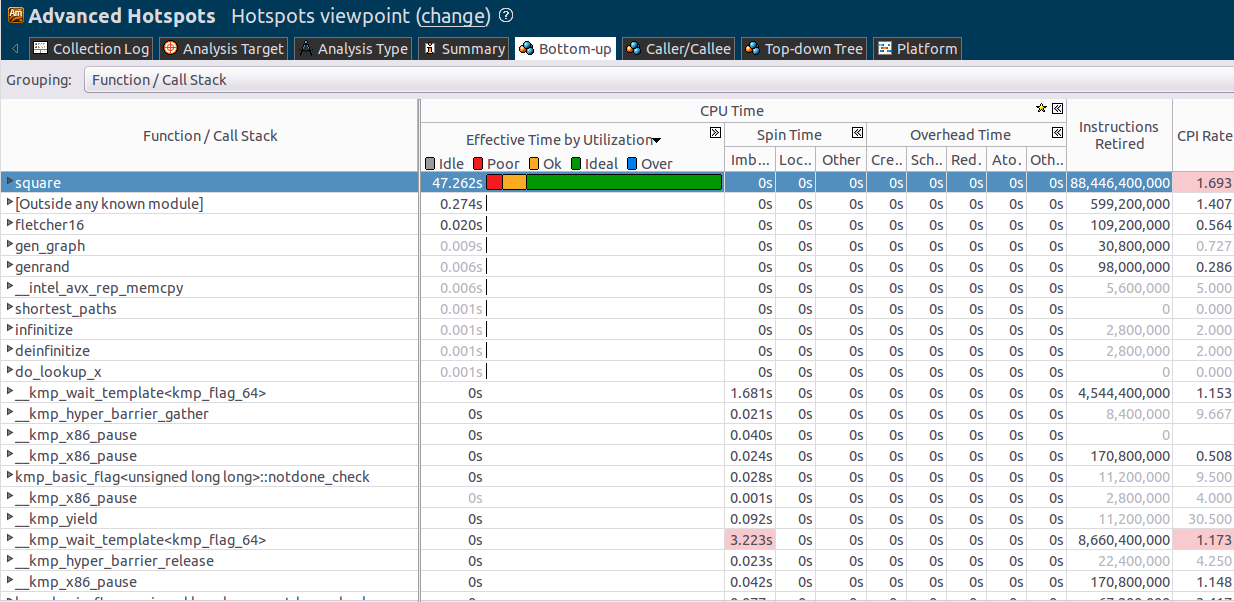
\includegraphics[width=0.8\textwidth]{figs/0_analysis.png}
    \caption{Initial Profile Analysis}
    \label{initial_profile_result_0}
\end{figure}

\begin{figure}[h]
    \centering
    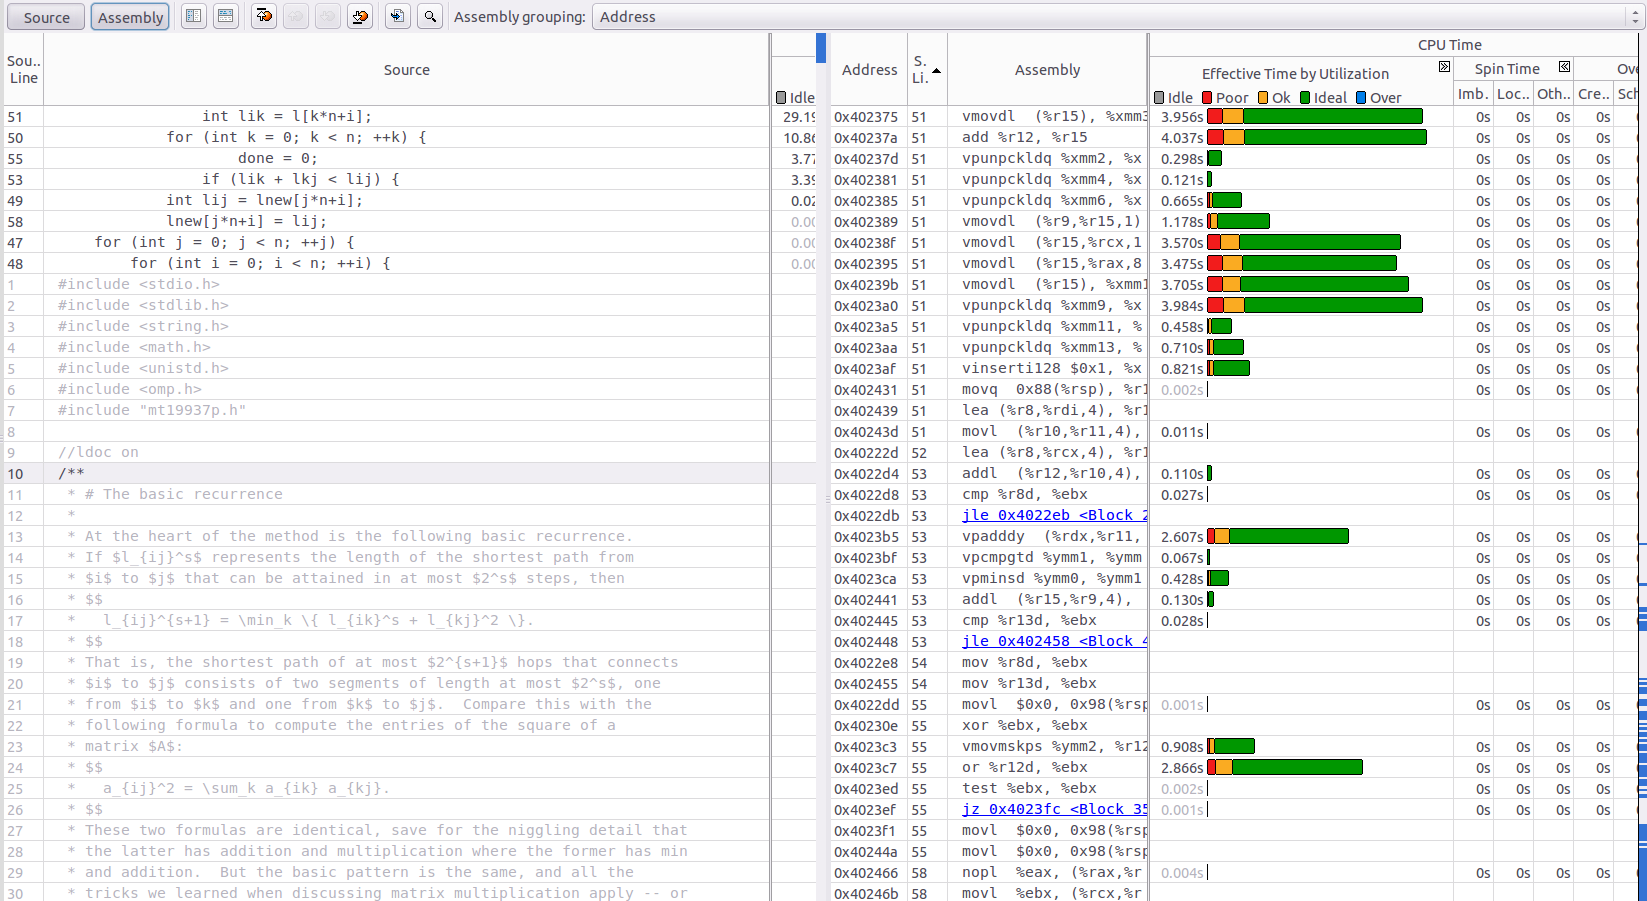
\includegraphics[width=0.8\textwidth]{figs/0_assembly.png}
    \caption{Initial Assembly Result}
    \label{initial_profile_result_1}
\end{figure}

\subsection{Initial Timing Result}

Initial timing result is shown in Figure \ref{initial_profile_result_2}. As we
can see the program is running with 8 threads using OpenMP and it takes 11.0818
seconds for 2000 nodes.

\begin{figure}[h]
    \centering
    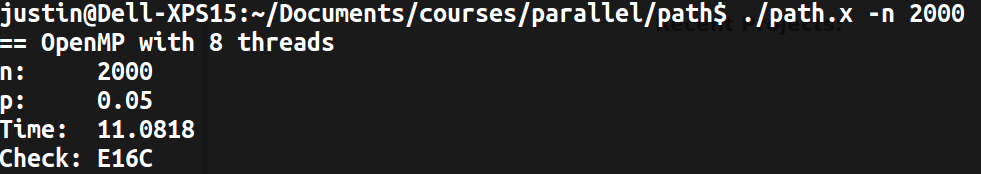
\includegraphics[width=0.8\textwidth]{figs/0_timing.png}
    \caption{Initial Timing Result}
    \label{initial_profile_result_2}
\end{figure}


\section{Vectorization}\label{sec:vectorization}
Vect...

%\section{Parallelization}\label{sec:parallel}
Parallel..

\section{Evaluation}\label{sec:evaluation}
%Justin%
\subsection{Timing After Vectorization}

\begin{figure}[H]
    \centering
    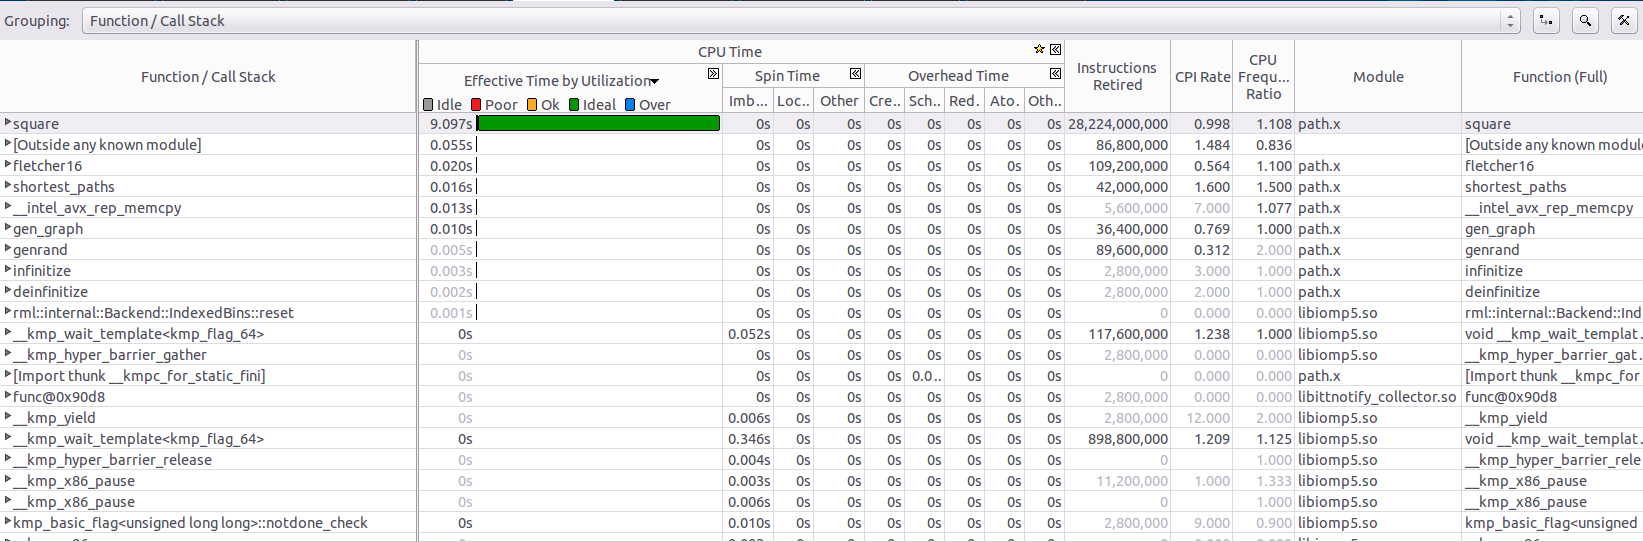
\includegraphics[width=0.8\textwidth]{figs/1_analysis.png}
    \caption{Profile Analysis After Vectorization}
    \label{vectorized_profile_result_0}
\end{figure}

As show in the picture, for the same problem size, the function \texttt{square} is more than 5
times faster than it was before, when we are running it with in Vtune, where one core is used to
trace other threads. In fact, running it with command line and time it with build in function
\texttt{omp\_get\_time()} shows the saving gives us a factor of more than 9 times faster.

\begin{figure}[H]
    \centering
    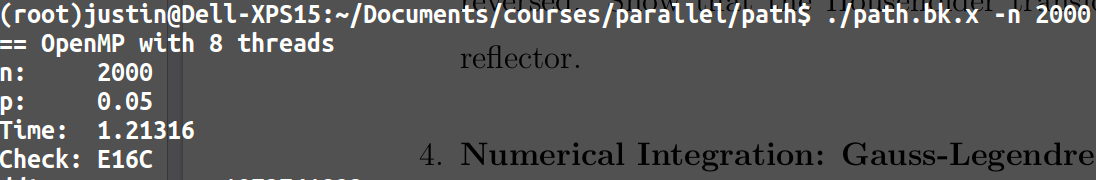
\includegraphics[width=0.8\textwidth]{figs/1_timing.png}
    \caption{Timing Result After Vectorization}
    \label{vectorized_profile_result_1}
\end{figure}

\begin{figure}[H]
    \centering
    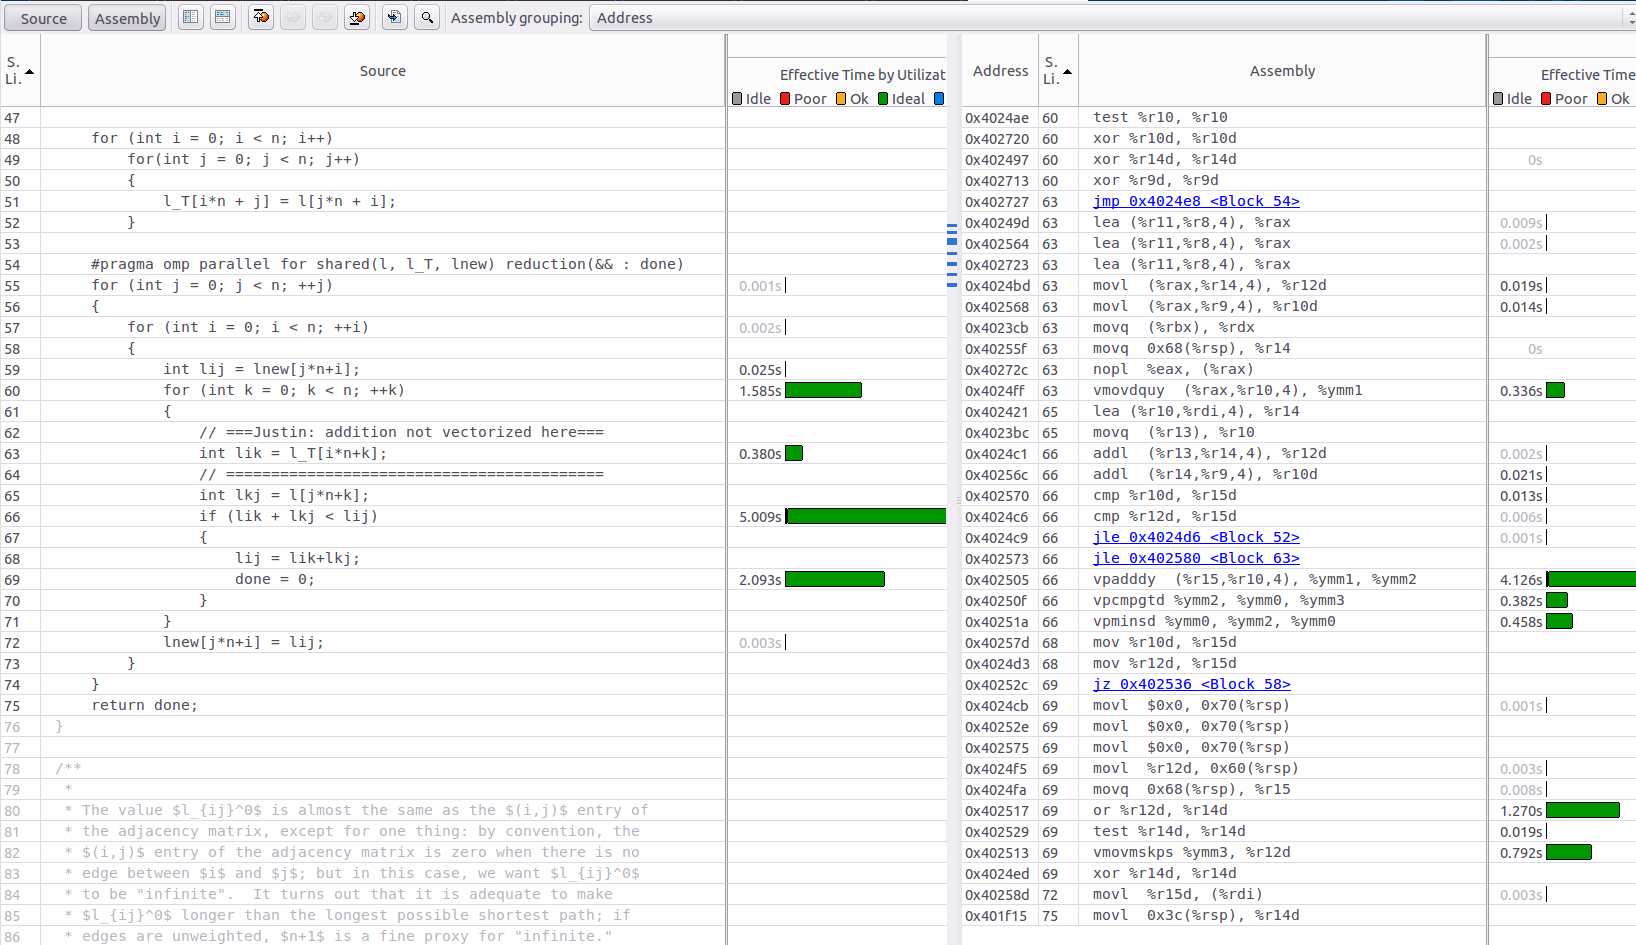
\includegraphics[width=0.8\textwidth]{figs/1_assembly.png}
    \caption{Assembly Analysis After Vectorization}
    \label{vectorized_profile_result_2}
\end{figure}

The assembly analysis is more informative as it tells how well our functions have been vectorized
as well as the timing. From the assembly analysis after vectorization, we can tell that the computations
in the inner has been vectorized. Which is where the savings come from.



\subsection{Data-Type Optimization}
As we went through tests, we found that the maximum distance between two vertices is
always below 20, even when we are calculating a 10000 by 10000 graph. Then it naturally
follows that, we don't necessarily need a 4-byte \textcolor{blue}{int} to store the
distance information. \\

To fit more data into register so that we can carry out more operation per cycle, we used
a prototype called \textcolor{blue}{ddt}, which can be any data type such as \textcolor{blue}{long},
\textcolor{blue}{short}, and \textcolor{blue}{char}. In fact, this gives us 30\% saving when we are
using \textcolor{blue}{char} to store the distance between two vertices. \\

Notice in Figure 8, we printed out a variable called \texttt{ddt\_upper\_range} which tells us the largest
distance we can have, in order to use one certain data-type. In the case with \textcolor{blue}{char}, the
largest distance is 127, which is proved to be more than enough by our tests.



\subsection{Midterm Profile Result}

\begin{figure}[H]
    \centering
    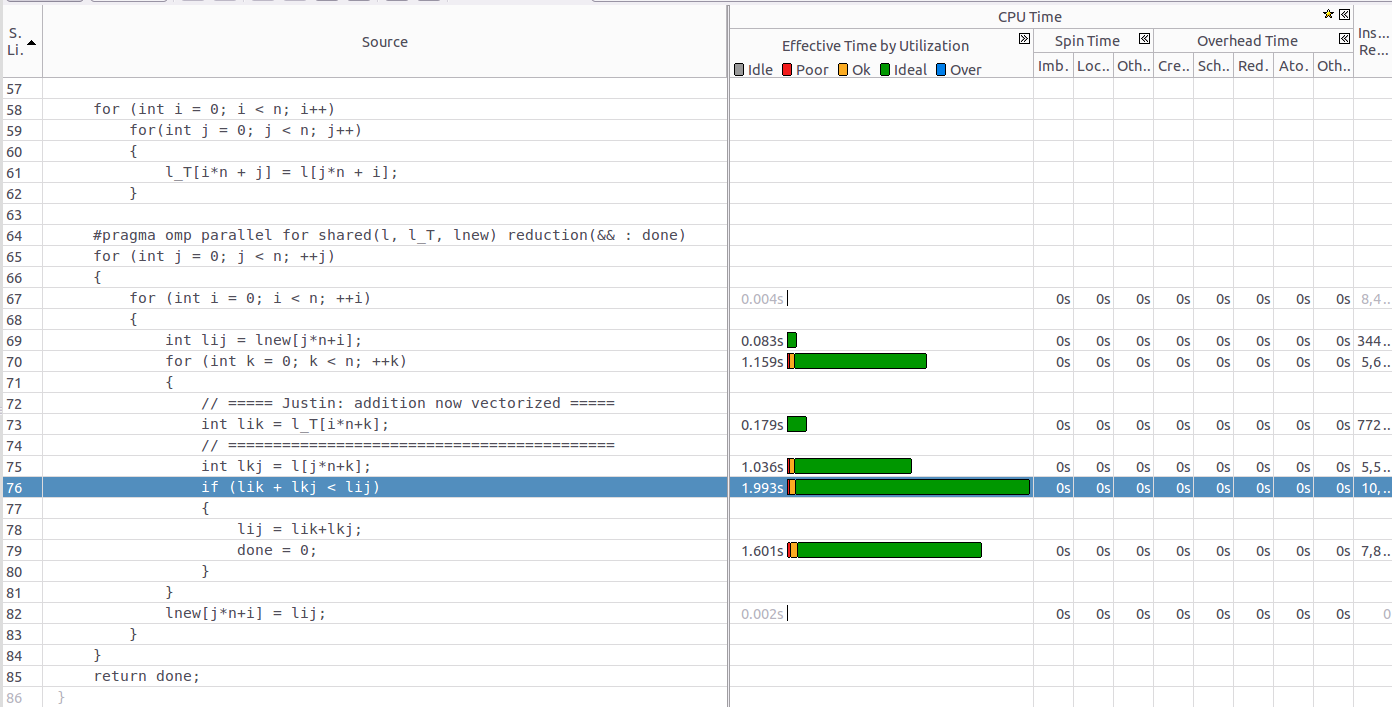
\includegraphics[width=0.8\textwidth]{figs/2_assembly.png}
    \caption{Initial Assembly Result}
    \label{ddt_profile_result_1}
\end{figure}

The assembly analysis after using data-type \textcolor{blue}{char} is down below. Comparing with Figure
\ref{vectorized_profile_result_2}, we can tell that the major saving comes from the addition between 
\texttt{lij} and \texttt{ljk}, which consist with what we would expect, since we can now fit more additions
into vector register to be calculated in one cycle.



\subsection{Initial Timing Result}

\begin{figure}[H]
    \centering
    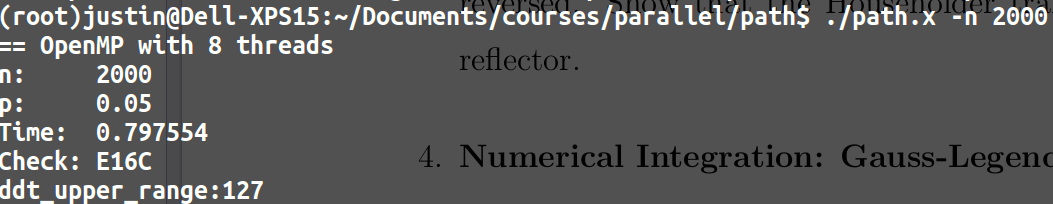
\includegraphics[width=0.8\textwidth]{figs/2_timing.png}
    \caption{Midterm Timing Result}
    \label{ddt_profile_result_2}
\end{figure}

Midterm timing result is shown in Figure \ref{ddt_profile_result_2}. As we
can see the program is running with 8 threads using OpenMP and it takes 0.7976
seconds for 2000 vertices.


\section{Summary}\label{sec:summary}

In this project, we did the following:

\begin{enumerate}
\item Profiled to find the hotspots, look into the vectorization report.
\item Optimized our code based on our finding, get a factor of more than 10.
\item Successfully parallel our code through MPI, board-cast algorithm, get the right answer.
\item Use non-blocking communication to speed up the MPI code.
\item Build up a mode to analysis the performance of our MPI code in terms of strong scaling and MPI
	  efficiency.
\end{enumerate}

From our result, we learned:

\begin{enumerate}
\item Non-blocking communication can help speed up the program, but it might not be that ideal.
\item When the size of a job is not large enough, the efficiency of MPI calculation maybe influenced.
\end{enumerate}
\end{document}
